\begin{usecase}{Receive Event Notifications}
    \ucbasicinfo{High}{Regular}
    \ucshortdescription{Users receive notifications about upcoming events.}
    \uctrigger{The UC is triggered when the choosen time of an event's reminder has arrived}
    \ucactors{User}{None}
    \ucpreconditions{User must be logged into the system and set a reminder of the specific event.}
    \ucrelationships{N/A}{N/A}{N/A}
    \ucinputsoutputs{
      \begin{itemize}
        \item \textbf{Time of the event reminder} (Source: User)
      \end{itemize}
    }{
      \begin{itemize}
        
        \item \textbf{Notifications sent to users.} (Destination: System)
      \end{itemize}
    }
    \ucmainflow{
      \begin{enumerate}
          \item The system checks the alarms set for every event.
        \ucinfo{The system checks every 1 minute for set alarms for every event.}      
        \item Notifications sent to users.
        \ucinfo{The user is reminded about the event by sending the notification}
      \end{enumerate}
    }
    \ucalternateflows{
      \begin{itemize}
        \item \textbf{If user denys the access to the notification the notifications are not sent.} 
      \end{itemize}  
    }
    \ucexceptions{
      \begin{itemize}
        \item \textbf{Netwok issue} 
      \end{itemize}
    }
    \ucconclusion{The system checks for set alarm every 1 minute and if the event is detected the system sends the notification.}
    \ucpostconditions{Notifications are sent.}
    \ucspecialrequirements{Notification permission.}
    \ucbusinessrules{The system has to check every minute for the set alarm.
    }
\end{usecase}

\begin{figure}[!h]
  \centering
  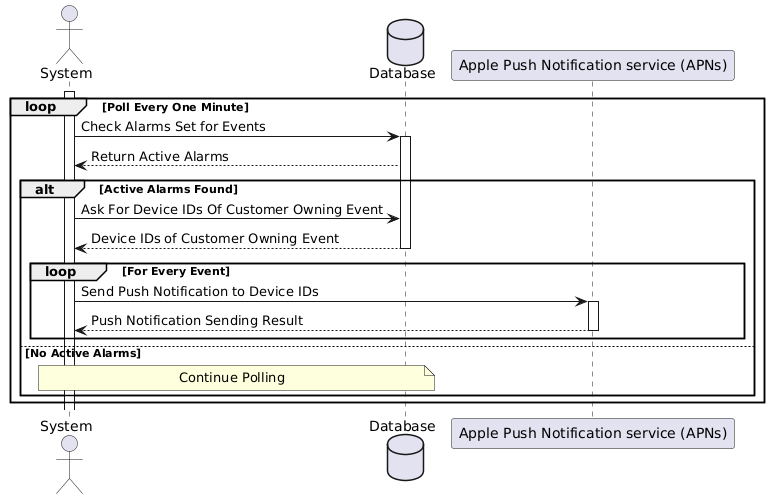
\includegraphics[width=\textwidth]{images/docs/diagrams/sequence-diagrams/all-sequence-diagrams/Receive Event Notifications.png}
  \caption{Receive Event Notifications Sequence Diagram}
  \label{fig:seq/receive-event-notifications}
\end{figure}